\documentclass[12pt]{article}

\usepackage{amsmath, amssymb, amsthm, enumerate, graphicx}
\usepackage[usenames,dvipsnames]{color}
\usepackage{bm}
\usepackage[colorlinks=true,urlcolor=blue]{hyperref}
\usepackage{geometry}
\geometry{margin=1in}
\usepackage{float}
\usepackage{graphics}
\setlength{\marginparwidth}{2.15cm}
\usepackage{booktabs}
\usepackage{enumitem}
\usepackage{epsfig}
\usepackage{setspace}
\usepackage{parskip}
\usepackage[normalem]{ulem}
\usepackage{tikz}
\usetikzlibrary{positioning, arrows, automata}
\usepackage{pgfplots}
\usepackage[font=scriptsize]{subcaption}
\usepackage{float}
\usepackage[]{algorithm2e}
\usepackage{environ}
\usepackage{bbm}
\usepackage{graphicx}
\usepackage{titling}
\usepackage{url}
\usepackage{xcolor}
\usepackage{lipsum}
\usepackage{lastpage}
\usepackage[colorlinks=true,urlcolor=blue]{hyperref}
\usepackage{multicol}
\usepackage{tabularx}
\usepackage{comment}
\usepackage[utf8]{inputenc}
\usepackage{amssymb}
\usepackage{setspace}
\usepackage{marvosym}
\usepackage{wrapfig}
\usepackage{datetime}
\usepackage[many]{tcolorbox}
\usepackage{array}
\usepackage{multirow}
\usepackage{wasysym}
\usepackage{cancel}

\usepackage{listings}
\usepackage{color}
\usepackage[thinlines]{easytable}
\usepackage{lastpage}

\newcommand{\R}{\mathbb{R}}
\newcommand{\blackcircle}{\tikz\draw[black,fill=black] (0,0) circle (1ex);}
\renewcommand{\circle}{\tikz\draw[black] (0,0) circle (1ex);}


\usetikzlibrary{positioning,calc}


%-------------------------------------------------------------------------------
% Custom commands
\usepackage{xcolor} %hilight
\newcommand{\hilight}[1]{\colorbox{yellow}{#1}}
%-------------------------------------------------------------------------------

\newtcolorbox[]{solution}[1][]{%
    breakable,
    enhanced,
    colback=white,
    title=Solution,
    #1
}
\begin{document}
\section*{}
\begin{center}
  \centerline{\textsc{\LARGE  Homework 4 Submission}}
\end{center}

Use this template to record your answers for Homework 4.  Add your answers using \LaTeX and then save your document as a PDF to upload to Gradescope.  You are required to use this template to submit your answers.  \textbf{You should not alter this template in any way} other than to insert your solutions.  You must submit all \pageref{LastPage} pages of this template to Gradescope.  Do not remove the instructions page(s).  Altering this template or including your solutions outside of the provided boxes can result in your assignment being graded incorrectly.

You should also export your code as a .py file and upload it to the \textbf{separate} Gradescope coding assignment. Remember to mark all teammates on \textbf{both} assignment uploads through Gradescope.

\section*{Instructions for Specific Problem Types}

On this homework, you must fill in blanks for each problem. Please make sure your final answer is fully included in the given space.  \textbf{Do not change the size of the box provided.}  For short answer questions you should \textbf{not} include your work in your solution.  Only provide an explanation or proof if specifically asked.

\begin{quote}
\textbf{Fill in the blank:} What is the course number?

\begin{tcolorbox}[fit,height=1cm, width=4cm, blank, borderline={1pt}{-2pt},nobeforeafter]
    \begin{center}\huge10-703\end{center}
    \end{tcolorbox}
\end{quote}

\newpage

\section*{Problem 0: Collaborators}
Enter your team members' names and Andrew IDs in the boxes below. If you worked in a team with fewer than three people, leave the extra boxes blank.

Name 1: \begin{tcolorbox}[fit,height=1cm, width=5cm, blank, borderline={1pt}{1pt},nobeforeafter]
    \begin{center}
    \vspace{3mm}
    \large{Mike Anoruo}
    \end{center}
\end{tcolorbox}
Andrew ID 1: \begin{tcolorbox}[fit,height=1cm, width=5cm, blank, borderline={1pt}{1pt},nobeforeafter]
    \begin{center}
    \vspace{3mm}
    \large{manoruo}
    \end{center}
\end{tcolorbox}
    \\
Name 2: \begin{tcolorbox}[fit,height=1cm, width=5cm, blank, borderline={1pt}{1pt},nobeforeafter]
    \begin{center}
    \vspace{3mm}
    \large{}
    \end{center}
\end{tcolorbox}
Andrew ID 2: \begin{tcolorbox}[fit,height=1cm, width=5cm, blank, borderline={1pt}{1pt},nobeforeafter]
    \begin{center}
    \vspace{3mm}
    %solution
    \end{center}
\end{tcolorbox} \\
Name 3: \begin{tcolorbox}[fit,height=1cm, width=5cm, blank, borderline={1pt}{1pt},nobeforeafter]
    \begin{center}
    \vspace{3mm}
    \large{}
    \end{center}
\end{tcolorbox}
Andrew ID 3: \begin{tcolorbox}[fit,height=1cm, width=5cm, blank, borderline={1pt}{1pt},nobeforeafter]
    \begin{center}
    \vspace{3mm}
    %solution
    \end{center}
\end{tcolorbox} \\
\vspace{0.5cm}
\vspace{0.5cm}

\newpage
\section*{Problem 1: CMA-ES (24 pts)}
\subsection*{1.1 Plot of CMA-ES on simple objective function (10 pts)}
\begin{tcolorbox}[fit,height=30em, width=40em, blank, borderline={1pt}{1pt},nobeforeafter]
            \begin{center}
                 \vspace*{5em}
                   \centering
                    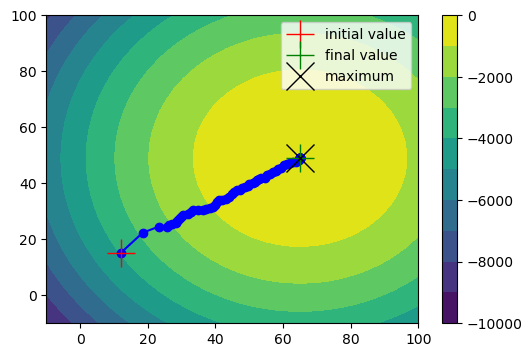
\includegraphics[width=0.6\textwidth]{visuals/CMA-ES_Simple.png}
            \end{center}
            \end{tcolorbox}
            
\subsection*{1.2 RL reward of fixed policies (4 pts)}

$x = (-1, -1, -1, -1, -1)$ : \begin{tcolorbox}[fit,height=1cm, width=5cm, blank, borderline={1pt}{1pt},nobeforeafter]
    \begin{center}
    \vspace{3mm}
    \large{15.6}
    \end{center}
\end{tcolorbox} \\
$x = (1, 0, 1, 0, 1)$ : \hspace{3.5em} \begin{tcolorbox}[fit,height=1cm, width=5cm, blank, borderline={1pt}{1pt},nobeforeafter]
    \begin{center}
    \vspace{3mm}
    \large{14.4}
    \end{center}
\end{tcolorbox} \\
$x = (0, 1, 2, 3, 4)$ : \hspace{3.5em} \begin{tcolorbox}[fit,height=1cm, width=5cm, blank, borderline={1pt}{1pt},nobeforeafter]
    \begin{center}
    \vspace{3mm}
    \large{9.4}
    \end{center}
\end{tcolorbox}

\subsection*{1.3 Plot of CMA-ES on Cartpole (10 pts)}
\begin{tcolorbox}[fit,height=30em, width=40em, blank, borderline={1pt}{1pt},nobeforeafter]
    \begin{center}
            \vspace*{5em}
            \centering
            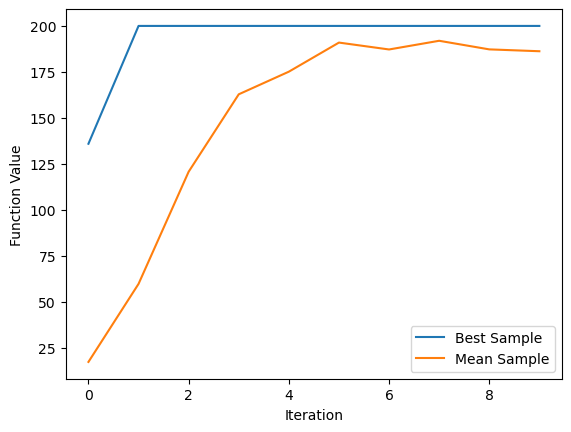
\includegraphics[width=0.6\textwidth]{visuals/CMA-ES_Cartpole.png}
    \end{center}
\end{tcolorbox}
    
\newpage

\subsection*{Problem 2: Imitation Learning (62 pts)}
\subsection*{Problem 2.1: BC (14 pts)}

\subsection*{2.1.1 Loss Plot + Final Loss Value BC (6 pts)}
\begin{tcolorbox}[fit,height=20em, width=40em, blank, borderline={1pt}{1pt},nobeforeafter]
     
      \centering
      \vspace*{0.8em}
    
    Final loss: loss 0.011179 
    \newline  
    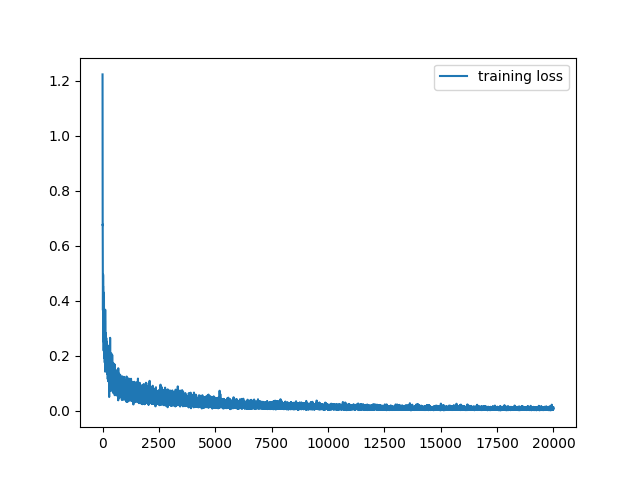
\includegraphics[width=0.6\textwidth]{visuals/BC_losses.png}
\end{tcolorbox}

\subsection*{2.1.2 Rewards Plot BC (6 pts)}

\begin{tcolorbox}[fit,height=24em, width=40em, blank, borderline={1pt}{1pt},nobeforeafter]
     \vspace*{5em}
    \centering
    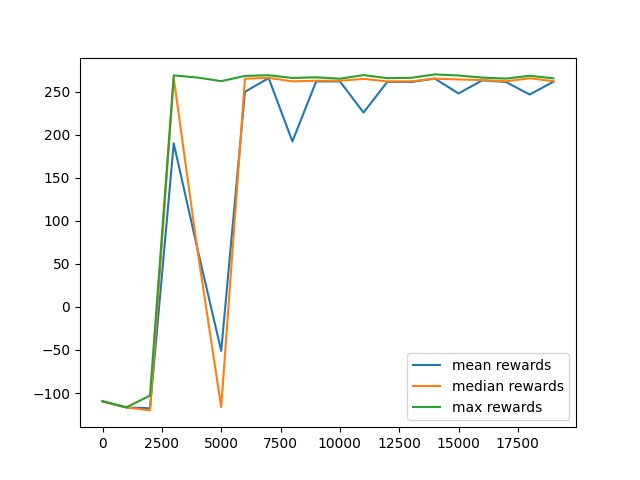
\includegraphics[width=0.6\textwidth]{visuals/BC_rewards.png}

\end{tcolorbox}
\subsection*{2.1.3 GIF link BC (2 pts)}

\begin{tcolorbox}[fit,height=5em, width=40em, blank, borderline={1pt}{1pt},nobeforeafter]
    \vspace*{1em}
    You can find this in my submission at:
    visuals/gifs\_BC.gif
\end{tcolorbox}

\subsection*{Problem 2.2: DAgger (18 pts)}

\subsection*{2.2.1 Loss Plot DAgger (6 pts)}
\begin{tcolorbox}[fit,height=20em, width=40em, blank, borderline={1pt}{1pt},nobeforeafter]
    \begin{center}
        \vspace*{2em}
        Final Loss: loss 0.005250
        \newline
        \centering
        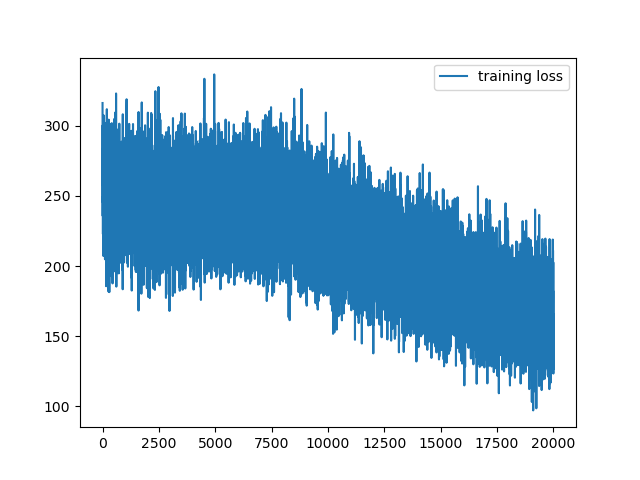
\includegraphics[width=0.5\textwidth]{visuals/DAgger_losses.png}
    \end{center}
\end{tcolorbox}
           
            
\subsection*{2.2.2 Rewards Plot DAgger (6 pts)}

\begin{tcolorbox}[fit,height=24em, width=40em, blank, borderline={1pt}{1pt},nobeforeafter]
    \begin{center}
        \vspace*{2em}
        \centering
        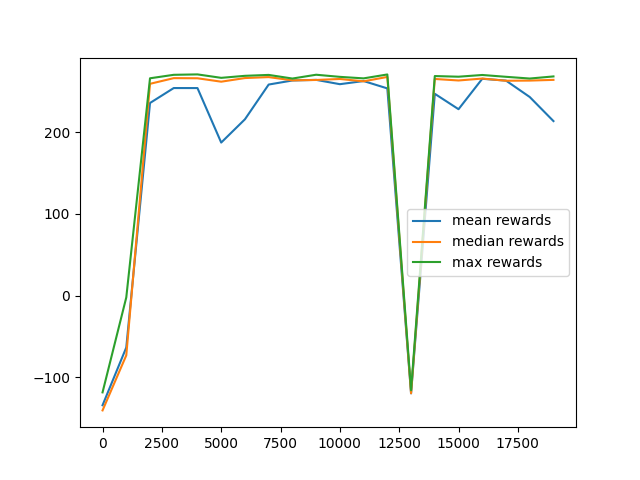
\includegraphics[width=0.6\textwidth]{visuals/DAgger_rewards.png}
    \end{center}
\end{tcolorbox}

\subsection*{2.2.3 GIF link DAgger (2 pts)}

\begin{tcolorbox}[fit,height=5em, width=40em, blank, borderline={1pt}{1pt},nobeforeafter]
    \vspace*{1em}
    You can find this in my submission at:
    visuals/gifs\_DAgger.gif
\end{tcolorbox}

\subsection*{2.2.4 Compare DAgger training with BC (written, 4 pts)}
\begin{tcolorbox}[fit,height=10em, width=40em, blank, borderline={1pt}{1pt},nobeforeafter]
            \begin{center}
            \vspace*{2em}
            DAgger worked better than BC because it continually queries the expert on the states the policy visits, correcting errors and reducing compounding mistakes, whereas BC only learns from the expert’s demonstration distribution and suffers from distribution shift.
            \end{center}
            \end{tcolorbox}

\newpage
\section*{Problem 2.3: Diffusion Policy (30 pts)}

\subsection*{2.3.1 Loss Plot + Final Loss value Diffusion Policy (6 pts)}
\begin{tcolorbox}[fit,height=30em, width=40em, blank, borderline={1pt}{1pt},nobeforeafter]
    \vspace*{2em}   
    \begin{center}
        Final loss = 0.03161560744047165
    \newline
    \centering
    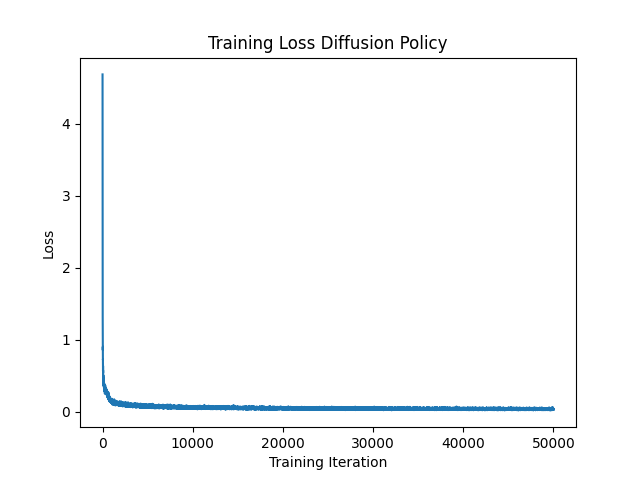
\includegraphics[width=0.6\textwidth]{visuals/diffusion_policy_loss_3_actions_in_a_row.png}
     
    \end{center}     
   
            \end{tcolorbox}


\subsection*{2.3.2 Rewards Diffusion Policy (15 pts)}
\subsection*{2.3.2.1; 3 actions evaluated in a row (5 pts)}

avg trajectory time: \begin{tcolorbox}[fit,height=1cm, width=2cm, blank, borderline={1pt}{1pt},nobeforeafter]
    \begin{center}
    \vspace{3mm}
    \large{845.33}
    \end{center}
\end{tcolorbox}
mean: \begin{tcolorbox}[fit,height=1cm, width=2cm, blank, borderline={1pt}{1pt},nobeforeafter]
    \begin{center}
    \vspace{3mm}
    \large{201.87}
    \end{center}
\end{tcolorbox}
median: \begin{tcolorbox}[fit,height=1cm, width=2cm, blank, borderline={1pt}{1pt},nobeforeafter]
    \begin{center}
    \vspace{3mm}
    \large{259.39}
    \end{center}
\end{tcolorbox}
max: \begin{tcolorbox}[fit,height=1cm, width=2cm, blank, borderline={1pt}{1pt},nobeforeafter]
    \begin{center}
    \vspace{3mm}
    \large{266.60}
    \end{center}
\end{tcolorbox}
    \\

\subsection*{2.3.2.2; 2 actions evaluated in a row (5 pts)}

avg trajectory time: \begin{tcolorbox}[fit,height=1cm, width=2cm, blank, borderline={1pt}{1pt},nobeforeafter]
    \begin{center}
    \vspace{3mm}
    \large{806.03}
    \end{center}
\end{tcolorbox}
mean: \begin{tcolorbox}[fit,height=1cm, width=2cm, blank, borderline={1pt}{1pt},nobeforeafter]
    \begin{center}
    \vspace{3mm}
    \large{183.63}
    \end{center}
\end{tcolorbox}
median: \begin{tcolorbox}[fit,height=1cm, width=2cm, blank, borderline={1pt}{1pt},nobeforeafter]
    \begin{center}
    \vspace{3mm}
    \large{258.10}
    \end{center}
\end{tcolorbox}
max: \begin{tcolorbox}[fit,height=1cm, width=2cm, blank, borderline={1pt}{1pt},nobeforeafter]
    \begin{center}
    \vspace{3mm}
    \large{266.30}
    \end{center}
\end{tcolorbox}
    \\

    
\subsection*{2.3.2.3; 1 action evaluated in a row (5 pts)}
avg trajectory time: \begin{tcolorbox}[fit,height=1cm, width=2cm, blank, borderline={1pt}{1pt},nobeforeafter]
    \begin{center}
    \vspace{3mm}
    \large{865.83}
    \end{center}
\end{tcolorbox}
mean: \begin{tcolorbox}[fit,height=1cm, width=2cm, blank, borderline={1pt}{1pt},nobeforeafter]
    \begin{center}
    \vspace{3mm}
    \large{208.96}
    \end{center}
\end{tcolorbox}
median: \begin{tcolorbox}[fit,height=1cm, width=2cm, blank, borderline={1pt}{1pt},nobeforeafter]
    \begin{center}
    \vspace{3mm}
    \large{259.27}
    \end{center}
\end{tcolorbox}
max: \begin{tcolorbox}[fit,height=1cm, width=2cm, blank, borderline={1pt}{1pt},nobeforeafter]
    \begin{center}
    \vspace{3mm}
    \large{264.89}
    \end{center}
\end{tcolorbox}
    \\

\subsection*{2.3.3 GIF link Diffusion Policy (2 pts)}

\begin{tcolorbox}[fit,height=5em, width=40em, blank, borderline={1pt}{1pt},nobeforeafter]
               \vspace*{1em}
    You can find this in my submission at:
    visuals/gifs\_diffusion.gif

\end{tcolorbox}
    
\subsection*{2.3.4 Compare diffusion policy and simple model runtime (written, 4 pts)}
\begin{tcolorbox}[fit,height=10em, width=40em, blank, borderline={1pt}{1pt},nobeforeafter]
            \begin{center}
            \vspace*{2em}

            The diffusion policy is slower because it generates each action through an iterative denoising process over many timesteps, whereas BC or DAgger output actions directly in a single forward pass.

            \end{center}
            \end{tcolorbox}
\subsection*{2.3.5 Compare diffusion policy with different actions in a row runtime (written, 3 pts)}
\begin{tcolorbox}[fit,height=10em, width=40em, blank, borderline={1pt}{1pt},nobeforeafter]
            \begin{center}
                \vspace*{2em}
                Predicting more actions at once reduces the number of diffusion model calls per trajectory, so trajectories with higher num\_actions\_to\_eval\_in\_a\_row run faster on average.
            \end{center}
            \end{tcolorbox}

\clearpage

\end{document}